\documentclass{standalone}

\usepackage{tikz}
\usepackage{pgf-umlcd}
\usepackage[bitstream-charter]{mathdesign} % +1! taules mes petites i hi caben
\usepackage[T1]{fontenc}
\usepackage[utf8]{inputenc}

\begin{document}

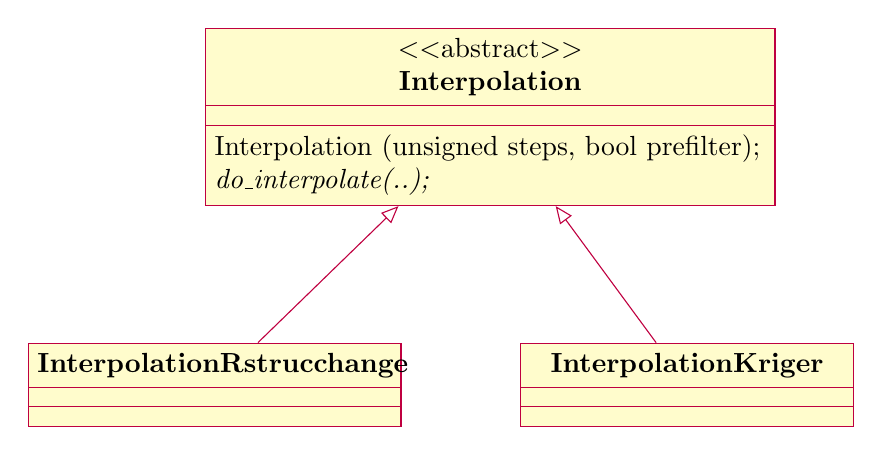
\begin{tikzpicture}

\begin{abstractclass}[text width=7cm]{Interpolation}{0,0}
\operation{Interpolation (unsigned steps, bool prefilter);}
\operation[0]{do\_interpolate(..);}
\end{abstractclass}

\begin{class}[text width=45mm]{InterpolationRstrucchange}{-3.5,-4}
\inherit{Interpolation}
\end{class}
\begin{class}[text width=40mm]{InterpolationKriger}{2.5,-4}
\inherit{Interpolation}
\end{class}
\end{tikzpicture}

\end{document}
